\chapter{The Proven Way to Have Your Best Year Ever}

This chapter reads Jim Rohn's seminar as a sequence of operational relations rather than as a loose string of aphorisms. Time outweighs money; sincerity does not certify truth; philosophy is the adjustable variable; repeated errors accumulate into failure, while repeated disciplines accumulate into change; results are read numerically; goals design the future; money is allocated by rule; words create light when they are prepared and measured. The source is an original Jim Rohn talk preserved in a curated LazyingArt LLC playlist rather than a formal classroom course, and no validated frame-backed equations survive for this lecture. Every display and diagram below is therefore a transcript-based reconstruction of the lecture's spoken formulas.

\section{Seminar Contract, Sincerity, and the Right to Be Taught}

\paragraph{The contract of the day.}
We begin where the speaker begins: with the price of attention. The audience has paid some money, but the real expenditure is a day of life. That is why the first principle is not motivation but valuation.

\begin{equation}
T > M,
\end{equation}

where \(T\) denotes time and \(M\) denotes money. We may replace money, but we do not replace the day. From this the lecture draws a practical demand: listen well, take notes, and insist that the day produce value.

\paragraph{Sincerity and truth.}
The next move is sharp and necessary. The lecture does not ask us to trust emotion blindly. It asks us to distinguish posture from truth.

\begin{equation}
\text{sincerity} \not\Rightarrow \text{truth}.
\end{equation}

One may be sincerely wrong. So the audience is asked to be student rather than disciple. Advice may be heard, processed, and tested, but action must become one's own.

\begin{equation}
\text{action} = \text{the product of one's own conclusion}.
\end{equation}

\paragraph{Autobiographical warrant.}
Only after this contract does Rohn justify why the audience should hear him at all. He gives the short story of obscurity, debt, embarrassment, Earl Shoaff, and disciplined change. The later formulas are therefore not offered as detached wisdom. They are offered as lived after-effects of a before-and-after experiment.

\paragraph{Ideas and receptivity.}
The room is also divided by receptivity. Some are willing to come, some are not; some hear and believe, some mock, some remain perplexed. The lecture does not resolve this mystery. It simply notes that teaching begins by sorting an audience, and that the audience now present must behave like students.

\section{From Blame to Philosophy: The First Piece of the Life Puzzle}

\paragraph{The controlling variable.}
Rohn's decisive claim is that philosophy is the major determining factor in how life works out. To state this carefully, let \(C\) denote the largely given conditions and let \(P\) denote personal philosophy.

\begin{definition}
In this lecture, \(C\) is the package of circumstances that arrives before any personal choice: seed, soil, rain, sunshine, seasons, economy, institutions, teachers, markets, and the surrounding people. The variable \(P\) is personal philosophy, the ``set of the sail,'' namely the pattern of interpretation and judgment by which one uses what has been given.
\end{definition}

The point is not that circumstances are unreal. The point is that they are not the speaker's preferred place to locate blame. We are told again and again that one may not curse seed, soil, rain, sunshine, the seasons, the economy, or the marketplace, because these are precisely the materials with which a life must be made.

\begin{equation}
C \approx \text{const}, \qquad \Delta P \Rightarrow \Delta R,
\end{equation}

where \(R\) denotes results.

\paragraph{The five pieces.}
The review of the ``life puzzle'' supplies the lecture's scaffold. It is not an even review. Philosophy is the governing term, while the remaining pieces are progressively more visible expressions of it.

\begin{figure}
\centering
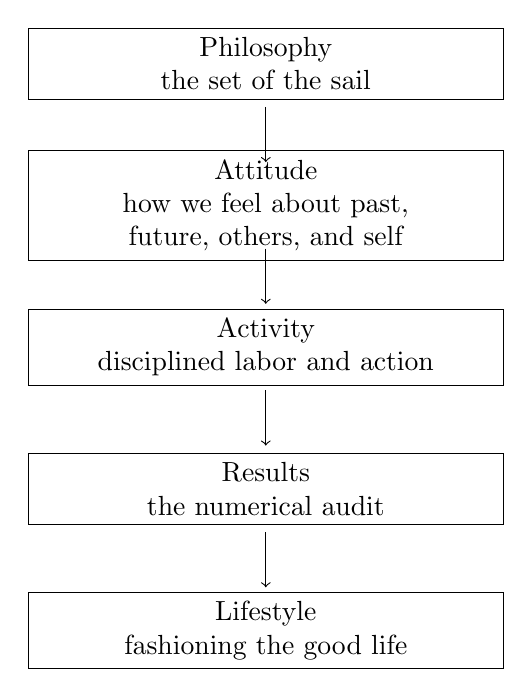
\begin{tikzpicture}[x=1cm,y=1cm]
\node[draw, text width=5.8cm, align=center] at (0,0) {Philosophy\\the set of the sail};
\node[draw, text width=5.8cm, align=center] at (0,-1.8) {Attitude\\how we feel about past, future, others, and self};
\node[draw, text width=5.8cm, align=center] at (0,-3.6) {Activity\\disciplined labor and action};
\node[draw, text width=5.8cm, align=center] at (0,-5.4) {Results\\the numerical audit};
\node[draw, text width=5.8cm, align=center] at (0,-7.2) {Lifestyle\\fashioning the good life};
\draw[->] (0,-0.55)--(0,-1.25);
\draw[->] (0,-2.35)--(0,-3.05);
\draw[->] (0,-4.15)--(0,-4.85);
\draw[->] (0,-5.95)--(0,-6.65);
\end{tikzpicture}
\end{figure}

\subsection{Question \& Answer}

\paragraph{Question.}
If the economy and circumstances stay roughly the same, how can a life change so much?

\paragraph{Answer.}
Because in the lecture the wind is not the sail. Rohn explicitly compares two six-year periods and says that government, taxes, economy, prices, and even negative relatives were ``about the same.'' Yet the second period no longer produced the first period's results. The changed term was not the weather of the world but the structure of judgment brought to it. Once philosophy changes, blame gives way to responsibility, and responsibility gives way to different daily action.

\section{Daily Errors, Daily Disciplines, and Accumulated Outcomes}

\paragraph{The two governing formulas.}
At this point the lecture tightens into its best-known pair of equations. They are verbal formulas, but they are precise enough to carry the entire chapter.

\begin{align}
\text{Failure} &= \text{a few errors in judgment} \\
&\quad \text{repeated every day}, \\
\text{Success} &= \text{a few simple disciplines} \\
&\quad \text{practiced every day}.
\end{align}

We are not being offered a theory of sudden catastrophe or sudden triumph. We are being offered a theory of accumulation.

\paragraph{A concrete mnemonic.}
The apple-versus-Hershey-bar sequence is not a nutritional treatise. It is a model of delayed causation. The same is true of the walk-around-the-block example. In each case the speaker chooses a small act whose penalty or reward does not fully show up on day one, precisely so that he can make the deeper point: delay in visible effect does not cancel cumulative effect.

\begin{proposition}
Delayed consequences do not cancel cumulative consequences.
\end{proposition}

\begin{proof}
The first omitted apple, or the first omitted walk, may produce no visible disaster at the end of the day. But the lecture insists that the absence of immediate punishment conceals rather than removes the cost. Repeat the omission for weeks, months, or years, and what was invisible locally becomes visible globally as illness, weak skill, or an empty bank account. The process is therefore cumulative even when it is not immediately dramatic.
\end{proof}

\paragraph{Mnemonic compression.}
The lecture then compresses the drift mechanism into a verbal update rule.

\begin{equation}
\text{could}+\text{should}+\text{don't}\Rightarrow \text{disaster}.
\end{equation}

And, by reversal,

\begin{equation}
\text{could}+\text{should}+\text{will}\Rightarrow \text{life change}.
\end{equation}

\subsection{Question \& Answer}

\paragraph{Question.}
If the needed discipline is simple, why do people still drift toward disaster?

\paragraph{Answer.}
Because easy-to-do is also easy-not-to-do. The first neglect is small, and the first delay seems harmless. The missing discipline produces no immediate collapse, so the mind falsely concludes that the omission does not matter. That is the trap. The speaker's whole point is that a simple neglect, repeated, writes a long future.

\paragraph{The stronger formulation.}
Rohn even sharpens ``don't'' into ``won't.'' At that point neglect is no longer mere carelessness. It has hardened into a philosophy.

\section{Attitude, Activity, Results, and Lifestyle}

\paragraph{Attitude.}
The remaining four pieces of the puzzle are treated more quickly, but they are not minor. Attitude is the configuration of feeling about the past, the future, other people, and oneself. The past must become a school rather than a club. The future must be designed well enough to create anticipation rather than apprehension. Others must be seen not as a nuisance but as the very material of market, family, community, and nation. The self must be valued enough to believe that change is possible.

\paragraph{Activity.}
The lecture then places activity at the center of causation. Wisdom alone does not perform a miracle, and neither does attitude alone. They become effective only when translated into labor.

\begin{equation}
\text{wisdom}+\text{attitude}+\text{disciplined labor}\Rightarrow \text{equity}.
\end{equation}

This is why the speaker calls activity the ``miracle-working piece.'' Seed, soil, sunshine, rain, and seasons are already in place. The human task is to plant, work, and persist.

\paragraph{Results.}
Results are the audit instrument. Here the lecture turns from exhortation to numbers. The manager who asked for ten calls in a week does not need a story; he needs a number. The teacher who asks how many books have been read, how many classes have been taken, or how much money has been saved and invested is not being cold. He is reading philosophy through measurable traces.

\begin{equation}
R=\bigl(\text{bank balance},\ \text{books read in 90 days},\ \text{classes taken in 6 months},\ \text{calls made in a week},\ \text{pounds overweight}\bigr).
\end{equation}

The lecture's slogan is exact enough to retain:

\begin{equation}
\text{success} = \text{a numbers game}.
\end{equation}

\begin{remark}
The ratios \(3:7\), \(3\%\), and \(5:95\) belong to the talk as rhetorical counts and lecture claims. They are structurally important because they sort behavior into minorities and majorities, but they should not be treated here as independently verified social statistics.
\end{remark}

\paragraph{Lifestyle.}
Lifestyle is the terminal form of the chain. It is not luxury for its own sake. It is the art of taking returns, values, and equities, then fashioning from them a ``good life.'' The word the lecture prefers is apt: we must fashion it, as one weaves a tapestry from disciplined returns.

\section{Personal Development and the Seasons of Life}

\paragraph{Work on the self.}
The lecture's middle movement is driven by one sentence from Shoaff:

\begin{equation}
\text{job-work}\Rightarrow \text{living}, \qquad \text{self-work}\Rightarrow \text{fortune}.
\end{equation}

This is the point at which philosophy becomes a program of self-development. The world is not asked to grow easier. The self is asked to grow more capable.

\paragraph{The seasonal model.}
Rohn's major metaphor is that life and business are like the seasons. This is not decorative. It is a compact model of recurrence. Winters come. Springs come. Summers require protection. Falls reveal what was actually planted and defended.

\begin{equation}
\text{You cannot change the seasons, but you can change yourself.}
\end{equation}

\begin{figure}
\centering
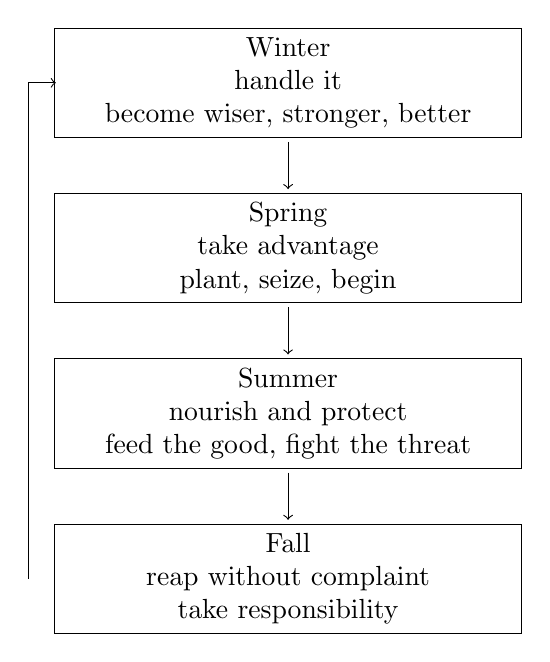
\begin{tikzpicture}[x=1cm,y=1cm]
\node[draw, text width=5.7cm, align=center] at (0,0) {Winter\\handle it\\become wiser, stronger, better};
\node[draw, text width=5.7cm, align=center] at (0,-2.1) {Spring\\take advantage\\plant, seize, begin};
\node[draw, text width=5.7cm, align=center] at (0,-4.2) {Summer\\nourish and protect\\feed the good, fight the threat};
\node[draw, text width=5.7cm, align=center] at (0,-6.3) {Fall\\reap without complaint\\take responsibility};
\draw[->] (0,-0.75)--(0,-1.35);
\draw[->] (0,-2.85)--(0,-3.45);
\draw[->] (0,-4.95)--(0,-5.55);
\draw[->] (-3.3,-6.3)--(-3.3,0)--(-2.95,0);
\end{tikzpicture}
\end{figure}

\paragraph{A one-sentence history.}
The lecture compresses human history itself into a single line: opportunity mixed with difficulty. That is why hoping for a world without winter is childish. The serious alternative is to become the kind of person who can handle winter, use spring, guard summer, and accept fall.

\paragraph{Worked example: the push-up sequence.}
The push-up example gives the lecture an explicit iterative model. We are asked whether ``the best you can do'' is the same as ``all you can do.'' The answer is no.

\begin{align}
N_0 &= 5, \\
N_1 &= N_0+5 = 10, \\
N_2 &= N_1+5 = 15, \\
N_3 &= N_2+5 = 20.
\end{align}

The arithmetic is schematic rather than physiological, but the argument is exact. A person who can presently do only \(5\) push-ups may, by short work-rest cycles, move far beyond the first apparent limit. The lecture's moral is that present capacity is not total capacity.

\paragraph{Rest as necessity.}
This is why rest is treated carefully. Rest is permitted, even required, but it is not to become the objective. The objective is action. Rest is a support for renewed action.

\section{Library, Journal, Reflection, Action, and the Five Abilities}

\paragraph{The machinery of self-education.}
After the seasons, the lecture becomes procedural. We are told to build a library, keep a journal, capture photographs, and stop trusting memory with important things. The library is evidence of seriousness; the journal is the place where lessons become portable; pictures rescue the event from disappearance.

\paragraph{The five abilities.}
Rohn then names a sequence of abilities that operationalizes personal development.

\begin{enumerate}
\item Absorb: do not miss the atmosphere, color, words, or event.
\item Respond: let experience touch the emotions as well as the intellect.
\item Reflect: return to the day, the week, the month, and the year.
\item Act: translate hot idea and strong feeling into immediate discipline.
\item Share: pass the lesson on so that it deepens in the speaker as well as in the hearer.
\end{enumerate}

\paragraph{Reflection as retention.}
Reflection is not nostalgia. It is the act of making the past more usable. The lecture recommends a rhythm: a few minutes at the end of the day, a few hours at the end of the week, half a day at the end of the month, and a larger review at the end of the year. This is how experience becomes future capital rather than lost time.

\paragraph{Action and diminishing intent.}
The fourth ability receives the most direct warning. When the idea is clear and the emotion is strong, one must act before the will cools.

\begin{equation}
\text{clear idea}+\text{strong emotion}+\text{delay}\Rightarrow \text{diminishing intent}.
\end{equation}

The law is simple: postponed insight decays. That is why the first book, the first note, the first walk, and the first phone call matter so much. A small discipline stabilizes an insight before it evaporates.

\paragraph{Discipline and self-respect.}
The lecture also connects discipline to self-worth. A small neglect does not merely lower external results. It erodes inner confidence. By the same token, a small discipline does not merely produce an isolated gain. It strengthens the whole person.

\begin{equation}
\text{affirmation without discipline}=\text{the beginning of delusion}.
\end{equation}

\paragraph{Sharing as enlargement.}
The last ability is not an afterthought. Sharing is itself a growth mechanism. If one idea is shared with \(n\) people, then the recipients hear it once, but the speaker hears it \(n\) times. Repetition enlarges the speaker's capacity.

\begin{equation}
\text{share with } n \text{ people} \Rightarrow \text{they hear it once, you hear it } n \text{ times}.
\end{equation}

\section{Goals, Financial Discipline, and Communication as Applied Form}

\paragraph{Goals as designed future.}
We now reach the lecture's future-design section. Goals are not mystical objects. They are written decisions. Without them the future is faced with apprehension; with them it may be faced with anticipation. The future is powerful not because it arrives automatically, but because a designed future changes today's step size.

\begin{equation}
\text{price is easy} \iff \text{promise is clear}.
\end{equation}

This is the connection between future and discipline. A person who clearly sees the promise will pay a price that would otherwise seem unbearable.

\paragraph{What a goal is really for.}
The famous millionaire example comes here. The lecture insists that the proper reason to set a large goal is not the money attached to it but the person required to reach it.

\begin{equation}
\text{value of a goal} = \text{what it makes of us}.
\end{equation}

This is the central reversal of the section. What we get matters, but what we become matters more. It is therefore a mistake to set goals too low, since a low goal asks for too little growth.

\paragraph{Marketplace value.}
The economic part begins with a clarification about pay. Time is necessary, but time alone is not what the market buys.

\begin{align}
\text{pay} &\neq \text{time alone}, \\
\text{pay} &= \text{value brought to the marketplace in a given time}.
\end{align}

Hence the possibility of advancement:

\begin{equation}
V_2=2V_1 \Rightarrow Y_2=2Y_1,
\end{equation}

where \(V\) is value and \(Y\) is income. If value doubles in the same interval, income may double in the same interval. This is why the lecture asks us to become more valuable rather than merely wait for a raise.

\paragraph{The 70/10/10/10 rule.}
The financial plan is presented as a discipline scheme for one dollar and then generalized upward. Let \(I\) be income, \(s\) spending, \(c\) charity, \(a\) active capital, and \(p\) passive capital. Then the lecture's ideal rule is

\begin{align}
s &\leq 0.70I, \\
c &= 0.10I, \\
a &= 0.10I, \\
p &= 0.10I.
\end{align}

A worked one-dollar example makes the rule concrete:

\begin{align}
I &= \$1.00, \\
s &= \$0.70, \\
c &= \$0.10, \\
a &= \$0.10, \\
p &= \$0.10.
\end{align}

And the warning attached to the plan is equally compact:

\begin{equation}
\text{outgo}>\text{income}\Rightarrow \text{upkeep becomes downfall}.
\end{equation}

\begin{remark}
The 70/10/10/10 rule is presented here as a moral-discipline plan, not as a complete modern investment framework. The lecture's interest is character, control, and habit formation.
\end{remark}

\paragraph{Profit, wages, and lending.}
The lecture makes two economic distinctions that should be preserved exactly.

\begin{equation}
\text{wages}\Rightarrow \text{living}, \qquad \text{profits}\Rightarrow \text{fortune}.
\end{equation}

Active capital means attempting to show a profit oneself. Passive capital means letting others use the capital and paying interest for the privilege. The moral position of power is therefore not that of spender but of lender:

\begin{equation}
\text{borrower}\Rightarrow \text{servant to lender}.
\end{equation}

The term ``profit'' is also broadened. It is monetary in one case, but in another it simply means leaving something better than one found it.

\paragraph{Strict accounts and new attitude.}
The lecture does not trust vague financial feeling. It asks for strict accounts. ``I don't know where it all goes'' is treated not as innocence but as indiscipline. The same is true of attitudes toward bills and taxes. To pay a bill is to reduce liabilities and increase assets; to pay taxes, in Rohn's rhetoric, is to feed the goose that lays the golden eggs.

\paragraph{Communication as outward form.}
The last movement widens from self-management to social effect. Words are powerful because they can move someone from darkness to sight. The lecture's four steps are straightforward:

\begin{enumerate}
\item Have something good to say.
\item Say it well.
\item Read the audience.
\item Use measured emotion.
\end{enumerate}

The distilled formula is

\begin{equation}
\text{effective communication}
=
\text{well-chosen words}
+
\text{measured emotion}.
\end{equation}

The speaker's point is not that words alone are enough. The words must be backed by learning, vocabulary, sensitivity, memory, and care. Then the social form of personal discipline appears: one human being speaks to another, and light is created.

\section{Summary}

The lecture's causal chain is simple and severe. Time must be treated as precious; sincerity must be separated from truth; philosophy must replace blame as the controlling variable; repeated errors and repeated disciplines must be understood as accumulative; results must be read numerically; self-development must proceed through seasons, books, journals, reflection, and action; the future must be written down; money must be ruled rather than merely spent; and communication must carry prepared thought with measured feeling. Nothing in this chapter depends on a better planet or a better season. Everything depends on what we do with what is already here.